%%%%%%%%%%%%%%%%%%%%%%%%%%%%%%%%%%%%%%%%%%%%%%%%%%%%%%%%%%%%%%%%%%%%%%%%%%%%%%%%
%2345678901234567890123456789012345678901234567890123456789012345678901234567890
%        1         2         3         4         5         6         7         8

\documentclass[letterpaper, 10 pt, conference]{ieeeconf}  % Comment this line out if you need a4paper

%\documentclass[a4paper, 10pt, conference]{ieeeconf}      % Use this line for a4 paper

\IEEEoverridecommandlockouts                              % This command is only needed if 
                                                          % you want to use the \thanks command

\overrideIEEEmargins                                      % Needed to meet printer requirements.

\usepackage{lmodern}
\usepackage{textcomp}
\usepackage{amsmath}
\usepackage{lipsum}
\usepackage{hyperref}
\usepackage{flushend}

\usepackage{graphicx}
\graphicspath{ {img/} }

\newcommand{\norm}[1]{\left\lVert#1\right\rVert}


\title{
Autonomous Forklift Implementation
}

\author{
Gudjon Einar Magnusson
\\ \href{mailto:gmagnusson@fc-md.umd.edu}{\tt\small gmagnusson@fc-md.umd.edu}
}

\begin{document}

\maketitle
\thispagestyle{empty}
\pagestyle{empty}


%%%%%%%%%%%%%%%%%%%%%%%%%%%%%%%%%%%%%%%%%%%%%%%%%%%%%%%%%%%%%%%%%%%%%%%%%%%%%%%%
\begin{abstract}

In this paper I present an implementation of an autonomous forklift uses a combination of task and motion planning to navigate in a warehouse-like environment and picks and places cargo pallets to satisfy a goal. The forklift uses propositional logic to plan high level task plans and then uses RRT to navigate as it performs each step of the plan.

\end{abstract}


%%%%%%%%%%%%%%%%%%%%%%%%%%%%%%%%%%%%%%%%%%%%%%%%%%%%%%%%%%%%%%%%%%%%%%%%%%%%%%%%
\section{Introduction}

Task planning and motion planning are both mature fields that offer a verity of advanced algorithms to solve their respective problems. These domains are generally studded in isolation by different people and surprisingly little consideration is given to the interaction between the two. It seams clear that any autonomous robot requires cooperation between task and motion planning.

Task planners can find a long sequence of actions to carry out a task under complex logical constraints. These planner abstract away the properties of the physical world they operate in.
Motion planners can find a optimal or near optimal path to move a physical object through space while avoiding collisions and respecting dynamic constraints. They generally operate over the time scale of a single task but do not consider the big picture.

In this paper I want to explicitly address how the two domains can be brought together in a single implementation. For demonstration I use an autonomous forklift operating in a warehouse-like environment. I believe this is a good example because it is fairly simple and intuitively shows the need for the combination of task and motion planning. Warehouse automation has also become one of the largest market for autonomous robotics

In section \ref{vehicle} I describe the details of the vehicle being used. I section \ref{task_planner} I describe the planning domain and the methods used for high level task planning. In section \ref{motion_planner} I describe the motion planning methods used to navigate. 

\label{vehicle}
\section{Vehicle Description}

\subsection{Vehicle Dynamics}
The vehicle is a standard forklift as one would expect to find in a warehouse. The forklift is driven by its two front wheels a turns using two back wheel. For this work I don't consider the full blown reverse Ackerman steering model, but instead use a simplified car model. The simplified model assumes instantaneous change in steering and velocity. The state of the vehicle can therefore be described by a 3 dimensional configuration space $(x, y, \theta)$, and the vehicle control is a 2 dimensional input vector $(v, s)$, where $v$ is the target velocity and $s$ is the steering angle.
The vehicle dynamics are described by the following equations:

\begin{align}
	\dot{x}	= v cos \theta \\ 
	\dot{y}	= v sin \theta \\
	\dot{\theta} = \frac{v}{L} \tan s
\end{align}

In addition to driving, the forklift is able to lift and lower its forks. For the purpose of navigation the state of the forks is not considered. The forks are considered to part of the forklifts footprint and are not allowed to overlap obsolesces in the environment. There are some scenarios were lifting the forks up to pass over obstacles would enable some solutions that would otherwise be impossible, but I concluded that this was not worth the effort. The one exception to this is when the forklift actually picks up a pallet. For that action the forks need to overlap the pallet as they are threaded through the holes on the pallet. This process is not controlled by the motion planner used for navigation, but instead uses a closed-loop controller that monitors the forklifts alignment with the pallet as it slowly moves forward.

\subsection{Simulation}

The forklift is implemented using the robot operating system (ROS) and Gazebo for simulation. For this work the planner uses perfect information read directly from the simulator, the problem of localization and sensing is not considered. It is assumed that the forklift has knowledge of its environment and its own position. Adding simultaneous localization and mapping (SLAM) for localization and vision for pallet identification has been considered for future work but will not be described here.

\subsection{Command Set}

The forklift can be controlled using 3 high level commands. Each command is implemented with a closed loop controller.

\paragraph{Move(Path)} Given a path (a list of positions) the forklift will follow the path as well as it can. If for any reason the forklift ends up to far off the path the action is canceled and return failure. 

\paragraph{Pickup(TargetPallet)} Given a target pallet the forklift will move carefully to thread the forks through the holes on the pallet. It is assumed that the forklift is already close to alignment with the pallet before the command is executed. If not it is likely to fail.

\paragraph{PutDown(TargetPose)} Given a target pose the forklift will carefully move to align with the pose such that it can lower a pallet it is holding down on the target pose. 

\label{task_planner}
\section{Task Planner}

Task planning for the forklift is performed using a STRIPS-like planner. The discrete state space is described using propositional logic and actions are described as a set of preconditions and a set of effects. The state space can be navigated by applying the effects of an applicable action to a state to get the next state. An action is applicable in a state if all of its preconditions are true in that state.
 
\subsection{Planning Domain}

\noindent\textbf{Objects:}
\begin{itemize}
  \item $Robots = \{forklift\}$
  \item $Pallets = \{pallet_1, pallet_2\}$
  \item $Stacks = \{stack_1, stack_2, stack_3\}$
\end{itemize}

\noindent\textbf{Predicates:}
\begin{itemize}
  \item $On(p, s)$, pallet $p$ is on stack $s$
  \item $Holding(r, p)$, Robot $r$ is holding pallet $p$
  \item $Empty(s)$, stack $s$ is empty
  \item $Aligned(r, s)$, robot $r$ is aligned to stack $s$
\end{itemize}

\noindent\textbf{Actions:}
\begin{itemize}
  \item $Align(r, s)$, move robot $r$ so it is aligned to stack $s$
  \begin{itemize}
  	\item[$pre:$] $\neg Aligned(r, s)$
  	\item[$eff:$] $Aligned(r, s)$
  \end{itemize}

  \item $Take(r, p, s)$, robot $r$ picks up pallet $p$ of stack $s$
  \begin{itemize}
  	\item[$pre:$] $Aligned(r, s)$, $Holding(r, None)$, $On(p, s)$
  	\item[$eff:$] $Holding(r, p)$, $\neg On(p, s)$, $Empty(s)$
  \end{itemize}

  \item $Put(r, p, s)$, robot $r$ puts pallet $p$ on stack $s$
  \begin{itemize}
  	\item[$pre:$] $Aligned(r, s)$, $Holding(r, p)$, $Empty(s)$
  	\item[$eff:$] $Holding(r, None)$, $On(p, s)$, $\neg Empty(s)$
  \end{itemize}
\end{itemize}


\subsection{Forward Search}

To construct a plan that reaches a given goal, the forklift uses breadth-first-search(BFS) to search a state graph from the start state until a state that satisfies the goal is found. BFS guaranties that the shortest solution is found, if one exists, but its not very efficient. The branching factor of this planning domain is quite high, especially as the number of pallets and stacks increases. To find a plan with 8 actions, involving 2 pallets and 3 stacks requires evaluating about 2800 nodes. 

\label{motion_planner}
\section{Motion Planner}

To perform actions the forklift needs to navigate from place to place. The motion planner plans a path for the forklift to follow from one pose to another, while respecting the kinematic constraints of the forklifts motion. This is implemented using the RRT algorithm.  

To be able to pick and place cargo pallets the forklift needs to arrive at a precise location and orientation so that the forks align with the holes on the pallet. Precisely connecting two poses in configuration space requires solving the two-point boundary value problem (two-point BVP). For a simplified car model like the forklift, the two-point BVP can be solved using Reeds-Shepp curves. Reeds-Shepp curves provide an optimal path for a car-like vehicle with a fixed turning radius and can move forward and backwards, as apposed to the Dubins curves that assume only forward motion. 

When planning a path the planner must account for obstacles in the workspace. Pallets are generally considered to be obstacles that must be avoided but unlike static obstacles like walls, their status can change depending on the state of the task. When the forklift picks up a pallet it is removed from the list of colliders in the workspace, when the pallet is put down the collider is added back.

\label{tamp}
\section{Task example}

\begin{figure}[h]
\centering
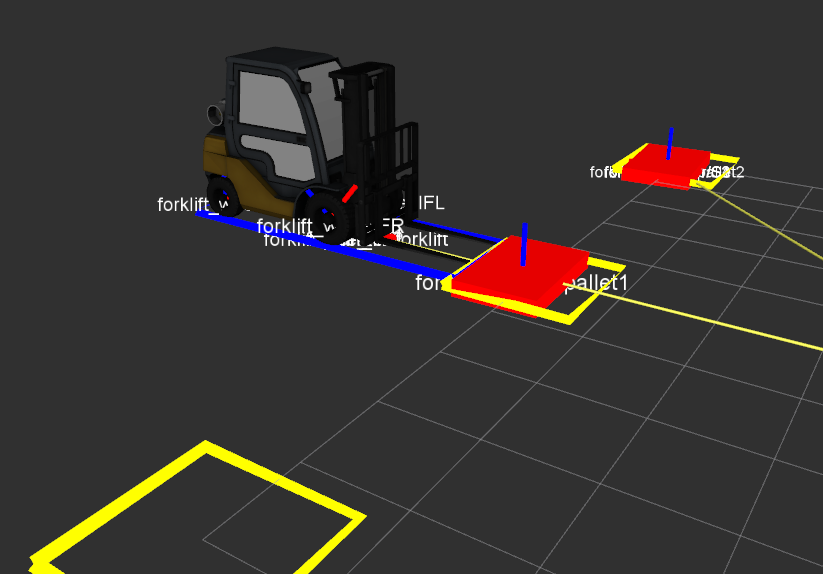
\includegraphics[width=0.4\textwidth]{forklift1}
\caption{The forklift working on a task involving 2 pallets and 3 stacks. Visualized in Rviz}
\label{fig:forklift1}
\end{figure}

A good example task is a two pallet swap using one extra stack for temporary storage. This scenario is shown in figure \ref{fig:forklift1} and is specified using the following start state and goal.

\noindent\textbf{Start State:}
\begin{itemize}
	\item $Holding(forklift, None)$
	\item $On(pallet1, stack1)$
	\item $On(pallet2, stack2)$
	\item $Empty(stack3)$
\end{itemize}

\noindent\textbf{Goal:}
\begin{itemize}
	\item $On(pallet1, stack2)$
	\item $On(pallet2, stack1)$
\end{itemize}

For this scenario the shortest plan that satisfies the goal involves 12 actions:

\begin{itemize}
	\item $Align(forklift, stack1)$
	\item $Take(forklift, pallet1, stack1)$
	\item $Align(forklift, stack3)$
	\item $Put(forklift, pallet1, stack3)$
	\item $Align(forklift, stack2)$
	\item $Take(forklift, pallet2, stack2)$
	\item $Align(forklift, stack1)$
	\item $Put(forklift, pallet2, stack1)$
	\item $Align(forklift, stack3)$
	\item $Take(forklift, pallet1, stack3)$
	\item $Align(forklift, stack2)$
	\item $Put(forklift, pallet1, stack2)$
\end{itemize}

To execute the plan returned by the task planner, each of the actions must be translated to a forklift command and executed one by one. For each move action the motion planner is called to plan a path.


\section{Conclusion}

In this paper I presented an autonomous forklift that uses a combination of task and motion planning. Unfortunately it does not address the problem of pickling arbitrary stack location to solve problems like initially wanted to do. 


%%%%%%%%%%%%%%%%%%%%%%%%%%%%%%%%%%%%%%%%%%%%%%%%%%%%%%%%%%%%%%%%%%%%%%%%%%%%%%%%


%\bibliography{ref}
\bibliographystyle{ieeetr}

\end{document}
